% GNUPLOT: LaTeX picture with Postscript
\begingroup
  \makeatletter
  \providecommand\color[2][]{%
    \GenericError{(gnuplot) \space\space\space\@spaces}{%
      Package color not loaded in conjunction with
      terminal option `colourtext'%
    }{See the gnuplot documentation for explanation.%
    }{Either use 'blacktext' in gnuplot or load the package
      color.sty in LaTeX.}%
    \renewcommand\color[2][]{}%
  }%
  \providecommand\includegraphics[2][]{%
    \GenericError{(gnuplot) \space\space\space\@spaces}{%
      Package graphicx or graphics not loaded%
    }{See the gnuplot documentation for explanation.%
    }{The gnuplot epslatex terminal needs graphicx.sty or graphics.sty.}%
    \renewcommand\includegraphics[2][]{}%
  }%
  \providecommand\rotatebox[2]{#2}%
  \@ifundefined{ifGPcolor}{%
    \newif\ifGPcolor
    \GPcolortrue
  }{}%
  \@ifundefined{ifGPblacktext}{%
    \newif\ifGPblacktext
    \GPblacktextfalse
  }{}%
  % define a \g@addto@macro without @ in the name:
  \let\gplgaddtomacro\g@addto@macro
  % define empty templates for all commands taking text:
  \gdef\gplbacktext{}%
  \gdef\gplfronttext{}%
  \makeatother
  \ifGPblacktext
    % no textcolor at all
    \def\colorrgb#1{}%
    \def\colorgray#1{}%
  \else
    % gray or color?
    \ifGPcolor
      \def\colorrgb#1{\color[rgb]{#1}}%
      \def\colorgray#1{\color[gray]{#1}}%
      \expandafter\def\csname LTw\endcsname{\color{white}}%
      \expandafter\def\csname LTb\endcsname{\color{black}}%
      \expandafter\def\csname LTa\endcsname{\color{black}}%
      \expandafter\def\csname LT0\endcsname{\color[rgb]{1,0,0}}%
      \expandafter\def\csname LT1\endcsname{\color[rgb]{0,1,0}}%
      \expandafter\def\csname LT2\endcsname{\color[rgb]{0,0,1}}%
      \expandafter\def\csname LT3\endcsname{\color[rgb]{1,0,1}}%
      \expandafter\def\csname LT4\endcsname{\color[rgb]{0,1,1}}%
      \expandafter\def\csname LT5\endcsname{\color[rgb]{1,1,0}}%
      \expandafter\def\csname LT6\endcsname{\color[rgb]{0,0,0}}%
      \expandafter\def\csname LT7\endcsname{\color[rgb]{1,0.3,0}}%
      \expandafter\def\csname LT8\endcsname{\color[rgb]{0.5,0.5,0.5}}%
    \else
      % gray
      \def\colorrgb#1{\color{black}}%
      \def\colorgray#1{\color[gray]{#1}}%
      \expandafter\def\csname LTw\endcsname{\color{white}}%
      \expandafter\def\csname LTb\endcsname{\color{black}}%
      \expandafter\def\csname LTa\endcsname{\color{black}}%
      \expandafter\def\csname LT0\endcsname{\color{black}}%
      \expandafter\def\csname LT1\endcsname{\color{black}}%
      \expandafter\def\csname LT2\endcsname{\color{black}}%
      \expandafter\def\csname LT3\endcsname{\color{black}}%
      \expandafter\def\csname LT4\endcsname{\color{black}}%
      \expandafter\def\csname LT5\endcsname{\color{black}}%
      \expandafter\def\csname LT6\endcsname{\color{black}}%
      \expandafter\def\csname LT7\endcsname{\color{black}}%
      \expandafter\def\csname LT8\endcsname{\color{black}}%
    \fi
  \fi
    \setlength{\unitlength}{0.0500bp}%
    \ifx\gptboxheight\undefined%
      \newlength{\gptboxheight}%
      \newlength{\gptboxwidth}%
      \newsavebox{\gptboxtext}%
    \fi%
    \setlength{\fboxrule}{0.5pt}%
    \setlength{\fboxsep}{1pt}%
    \definecolor{tbcol}{rgb}{1,1,1}%
\begin{picture}(7200.00,5040.00)%
    \gplgaddtomacro\gplbacktext{%
      \csname LTb\endcsname%%
      \put(814,704){\makebox(0,0)[r]{\strut{}$0$}}%
      \put(814,1218){\makebox(0,0)[r]{\strut{}$0.2$}}%
      \put(814,1733){\makebox(0,0)[r]{\strut{}$0.4$}}%
      \put(814,2247){\makebox(0,0)[r]{\strut{}$0.6$}}%
      \put(814,2762){\makebox(0,0)[r]{\strut{}$0.8$}}%
      \put(814,3276){\makebox(0,0)[r]{\strut{}$1$}}%
      \put(814,3790){\makebox(0,0)[r]{\strut{}$1.2$}}%
      \put(814,4305){\makebox(0,0)[r]{\strut{}$1.4$}}%
      \put(814,4819){\makebox(0,0)[r]{\strut{}$1.6$}}%
      \put(946,484){\makebox(0,0){\strut{}$0$}}%
      \put(1783,484){\makebox(0,0){\strut{}$1$}}%
      \put(2619,484){\makebox(0,0){\strut{}$2$}}%
      \put(3456,484){\makebox(0,0){\strut{}$3$}}%
      \put(4293,484){\makebox(0,0){\strut{}$4$}}%
      \put(5130,484){\makebox(0,0){\strut{}$5$}}%
      \put(5966,484){\makebox(0,0){\strut{}$6$}}%
      \put(6803,484){\makebox(0,0){\strut{}$7$}}%
      \colorrgb{0.58,0.00,0.83}%%
      \settowidth{\gptboxwidth}{\widthof{$\mu = 0.1$}}
	\advance\gptboxwidth by 2\fboxsep
      \savebox{\gptboxtext}{\parbox[c][\totalheight+2\fboxsep]{\gptboxwidth}{\centering{$\mu = 0.1$}}}
	\settowidth{\gptboxwidth}{\usebox{\gptboxtext}}
	\advance\gptboxwidth by 2\fboxsep
	\put(5130,1861){\makebox(0,0)[l]{\framebox[\gptboxwidth]{\usebox{\gptboxtext}}}}
      \colorrgb{0.00,0.62,0.45}%%
      \settowidth{\gptboxwidth}{\widthof{$\mu = 0.5$}}
	\advance\gptboxwidth by 2\fboxsep
      \savebox{\gptboxtext}{\parbox[c][\totalheight+2\fboxsep]{\gptboxwidth}{\centering{$\mu = 0.5$}}}
	\settowidth{\gptboxwidth}{\usebox{\gptboxtext}}
	\advance\gptboxwidth by 2\fboxsep
	\put(1615,3276){\makebox(0,0)[l]{\framebox[\gptboxwidth]{\usebox{\gptboxtext}}}}
    }%
    \gplgaddtomacro\gplfronttext{%
      \csname LTb\endcsname%%
      \put(209,2761){\rotatebox{-270}{\makebox(0,0){\strut{}$\left|f_t\right|$}}}%
      \put(3874,154){\makebox(0,0){\strut{}$f_n$}}%
      \csname LTb\endcsname%%
      \put(5816,4646){\makebox(0,0)[r]{\strut{}$\varepsilon_{yy} = 0\%$}}%
      \csname LTb\endcsname%%
      \put(5816,4426){\makebox(0,0)[r]{\strut{}$\varepsilon_{yy} = 11\%$}}%
    }%
    \gplbacktext
    \put(0,0){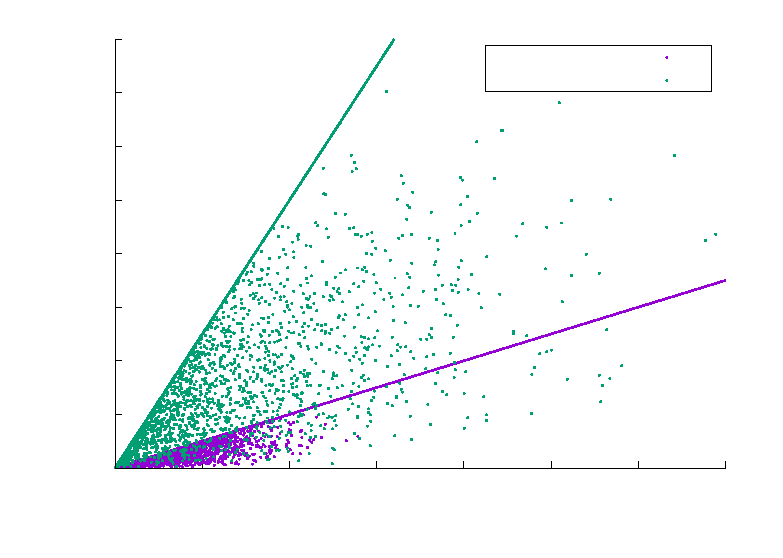
\includegraphics[width={360.00bp},height={252.00bp}]{./ConditionCoulomb}}%
    \gplfronttext
  \end{picture}%
\endgroup
